\subsection{Diferencia entre MCIS y MCES}

En el paper de Ehrlich and M. Rarey se introducen técnicas de comparación de grafos moleculares, haciendo referencia al problema del MCS (maximal common subgraph). Sin embargo, el paper se enfoca en un problema diferente al planteado en este trabajo.

El problema al que hace referencia el paper es el MCIS (\textit{Maximal common induced subgraph}), es decir, dados G1 = (V1 , E1) y G2 = (V2 , E2) encontrar un grafo maximal, isomorfo tanto a un subgrafo \textbf{inducido} de G1 como a un subgrafo \textbf{inducido} de G2. Mientras que el problema planteado en este trabajo es el MCES (\textit{Maximal common edge subgraph}), es decir, un grafo isomorfo tanto a un subgrafo de G1 como a un subgrafo de G2 que maximice la cantidad de aristas.

\begin{figure}[H]
 \centering
	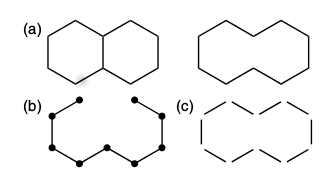
\includegraphics[width=0.7\textwidth]{img/problema1.png}
	\caption{MCIS versus MCES. Ejemplo presentado en el paper: (a) Molecular graph of
decalin (labels not shown). (b) Molecular graph of cyclodecane (labels
not shown). (c) MCIS of (a) and (b). (d) MCES of (a) and (b).}
	\label{fig:problema1-1}
\end{figure}

\subsection{Aplicaciones en la química}

Los algoritmos de MCS tienen varias aplicaciones en la ciencia molecular. En el paper se presentan varios tipos de aplicaciones: en la primera parte, se consideran algoritmos aplicados a grafos que representan moléculas orgánicas pequeñas, como drogas, mientras que en la segunda parte se mencionan aplicaciones en grafos derivados de moléculas más grandes como proteínas.

El problena del MCS es usado para medir similaridad estructural entre moléculas pequeñas, mientras que en moléculas más grandes se utilizan para calcular estructuras comunes entre moléculas. Además se menciona que a pesar de que es muy común intentar estudiar patrones comunes estructurales en moléculas de ARN (ácidos ribonucleicos), estos algoritmos no aplican demasiado.

\subsubsection{Moléculas orgánicas pequeñas}

Los algoritmos de MCS se utilizan para identificar familias de ligandos, predecir actividad de ligandos o analizar el mecanismo de reacciones. Otras aplicaciones implican alineación de ligandos, determinación de relaciones cuantitativas de propiedades estructurales y modelado farmacóforo. Algunos ejemplos son:

\begin{itemize}
\item \textbf{Clasificación de compuestos:}
Un problema central cuando se trata de pequeñas moléculas en la investigación farmacéutica es agrupar compuestos en familias o clusters según su relación estructural. Un MCS puede describir sub-estructuras comunes así como grupos funcionales entre dos moléculas. Utilizando un algoritmo para calcular el MCES se puede detectar similaridad entre compuestos que no comparten una gran sub-estructura común pero sí grupos funcionales no necesariamente conectados entre sí. A partir del número de vértices y ejes que comprende el MCS, se puede calcular un grado de similaridad entre moléculas.

\item \textbf{Predicción de actividad de compuestos:}
Una pieza clave para encontrar nuevas drogas es la identificación de compuestos químicos que muestren actividad en procesos biológicos específicos. Estudios muestran que compuestos estructuralmente similares suelen tener actividad similar, por lo que se busca identificarlos para reducir la cantidad de moléculas que deben ser testeadas experimentalmente. Las moléculas son representadas usando grafos y árboles donde los vértices representan grupos funcionales y los ejes la distribución topológica de los mismos. Se utiliza un promedio entre los valores de similaridad de los vértices comunes del MCIS entre dos compuestos para reflejar la similaridad entre las moléculas.

\item \textbf{Scaffold Hopping:}
Una desventaja de los métodos basados en similaridad para cribado virtual es su tendencia a identificar solamente compuestos que son estructuralmente similares. Sin embargo, es interesante encontrar moléculas que sean construidas desde diferentes andamios que aún preserven actividad contra el mismo tipo de proteína. Para eso se utilizan métodos de MCS sobre grafos reducidos que describen características escenciales para la actividad biológica.

\item \textbf{Mapeo de reacciones:}
Una reacción química transforma la molécula reactante al producto eliminando enlaces y formando nuevos. El método mencionado utiliza un modelado de reacciones como grafos moleculares donde los vértices son átomos y los ejes son enlaces, con pesos dados por la estabilidad de los enlaces. Usando un wMCES (weighted MCES o MCES con aristas con peso) que maximice la suma de ejes en común se puede determinar el conjunto de enlaces que fueron conservados durante la reacción con mayor probabilidad. Esto permite realizar un mapeo entre el reactivo y el producto.

\item \textbf{Determinación de relaciones cuantitativas de propiedades estructurales (QSAR):}
El concepto de QSAR es transformar conocimientos químicos en ecuaciones matemáticas que relacionen una estructura con una actividad o propiedad específica. Este modelo describe cada ligando usando valores de similaridad obtenidos por algoritmos de MCS.

\end{itemize}

\subsubsection{Proteinas}

\begin{itemize}
\item \textbf{Alineación estructural:}
La comparación estructural entre proteínas resulta muy útil para obtener información sobre la función, estabilidad y comportamiento general de las mismas. Al igual que en aplicaciones anteriores, las proteínas son modeladas con grafos y el MCES entre ellos se utiliza para describir la similaridad entre las mismas.

\item \textbf{Análisis de patrones estructurales:}
Se utiliza el MCIS para calcular la relación estructural entre dos proteínas. Esto permite investigar patrones estructurales entre proteínas relacionadas con funciones específicas.

\end{itemize}





